%*******************************************************************************
%****************************** Fifth Chapter *********************************
%*******************************************************************************

\chapter{Cosmic Muon Tomography}

\ifpdf
    \graphicspath{{Chapter5/Figs/Raster/}{Chapter5/Figs/PDF/}{Chapter5/Figs/}}
\else
    \graphicspath{{Chapter5/Figs/Vector/}{Chapter5/Figs/}}
\fi

\section{Overview}
Cosmic $\mu$ tomography is split into two distinct types two sided and one sided. Two sided cosmic $\mu$ is preferred if it is feasible this is because both attenuation and scattering can be measured when using this technique. The effect of the cosmic $\mu$ scattering can be seen in figure \ref{fig:twoSidedCosmicMuonTomographySchults} the cosmic $\mu$ which travel through the dense object will scatter more than the cosmic $\mu$ that don't. By making coincident measurements of the cosmic $\mu$ it is possible to find vertices using this method. This method is extremely powerful but can only be used for smaller objects in most cases. 
\\\\ For larger objects one sided cosmic $\mu$ tomography has to be used. An example of what one sided cosmic muon tomography looks like can be seen in figure \ref{fig:oneSidedCosmicMuonExample} when there is an object that can attenuate cosmic $\mu$ then the number of cosmic $\mu$ will decrease in the direction of the object being imaged. This method cannot measure scattering or vertices however that is still sufficient in many cases such as the imaging done by the DIAPHANE collaboration seen in figure  \ref{fig:diaphaneStructualImaging}. Which uses 4 different locations to image the La Soufriere of Guadeloupe dome and measure the density for volcanic observations \cite{Marteau_2017}.
\begin{figure}[H]
 \centering
 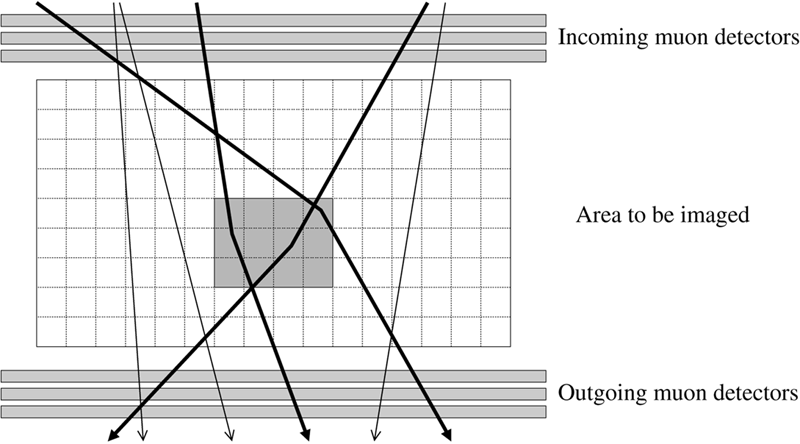
\includegraphics[width=0.8\linewidth]{Chapter5/Figs/Raster/twoSidedCosmicMuon_schults2007.png}
 \captionof{figure}{An side on view of two sided cosmic $\mu$ tomography the detectors are of similar size or larger than the object that is being measured in order to make coincided measurements using cosmic $\mu$ seen in the scattered (black) cosmic $\mu$ from \cite{schultz_2007}. }
 \label{fig:twoSidedCosmicMuonTomographySchults}
\end{figure}
 
 \begin{figure}[H]
 \centering
 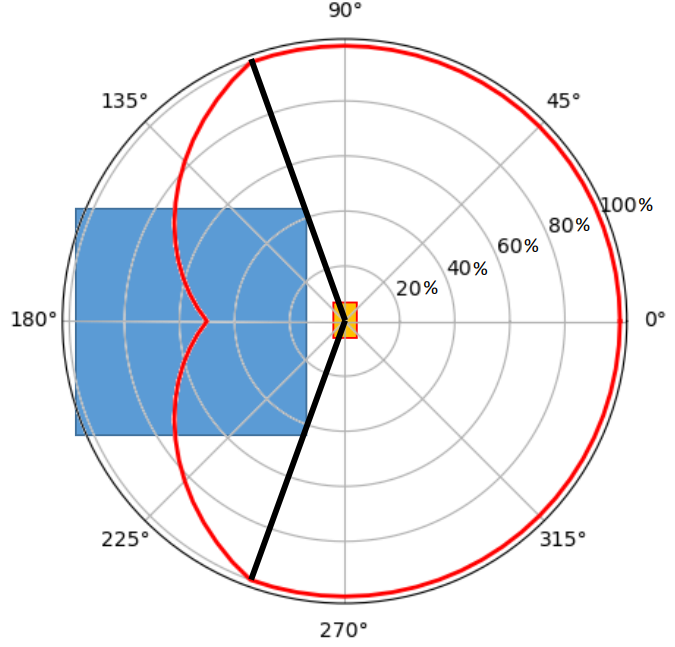
\includegraphics[width=0.6\linewidth]{Chapter5/Figs/Raster/oneSidedCosmicMuonExample.png}
 \captionof{figure}{An example of what one sided cosmic $\mu$ tomography looks like from a top down view. When there is an object that attenuates $\mu$ significantly the percentage of $\mu$ detected decreases in the direction of the object.}
 \label{fig:oneSidedCosmicMuonExample}
\end{figure}
 
\begin{figure}[H]
 \centering
 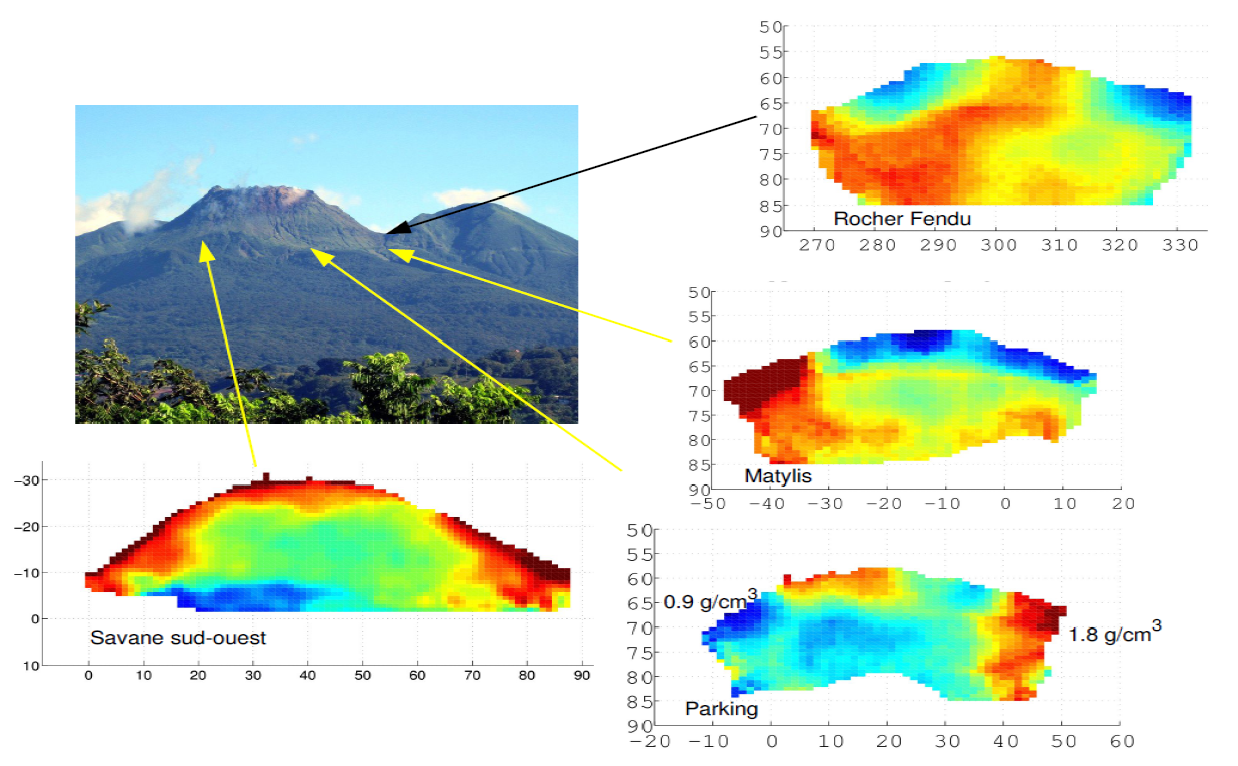
\includegraphics[width=1.0\linewidth]{Chapter5/Figs/Raster/diaphane_structuralImaging.png}
 \captionof{figure}{DIAPHANE structural imaging of the La Soufriere of Guadeloupe dome from 4 different acquisition sites around the dome. The blue areas are the less dense zones of the volcano. The red areas have the highest density. Average density extracted from all those images ranges from 1.6 to 1.8 g.cm$^{-3}$ from \cite{Marteau_2017}} %~can be used as a kind of place holder in latex
 \label{fig:diaphaneStructualImaging}
\end{figure}

\section{Deployment At Wylfa}\label{sec:deploymentAtWylfa}
The original prototype detector was deployed at the Wylfa Nuclear power station from 07-07-2014 to 25-02-2016 with data being taken continuously over that time period both with the reactor on and off with ibd measurements seen in figure \ref{fig:prototypeMeasumentFlux}. The placement of the detector in relation to the Wylfa reactor buildings can be seen in figure \ref{fig:wylfaTrace} the reactors were placed either end of the main reactor building in the centre of the cylindrical shaped ends. The overall shape of each of these buildings seen in figure \ref{fig:wylfaAir} causes the shape of the shadow to be quite different from what might be expected. The overall shadow in both $\theta$ and $\phi$ will therefore be an overlapping series of boxes rather than just one.   

\begin{figure}[H]
 \centering
 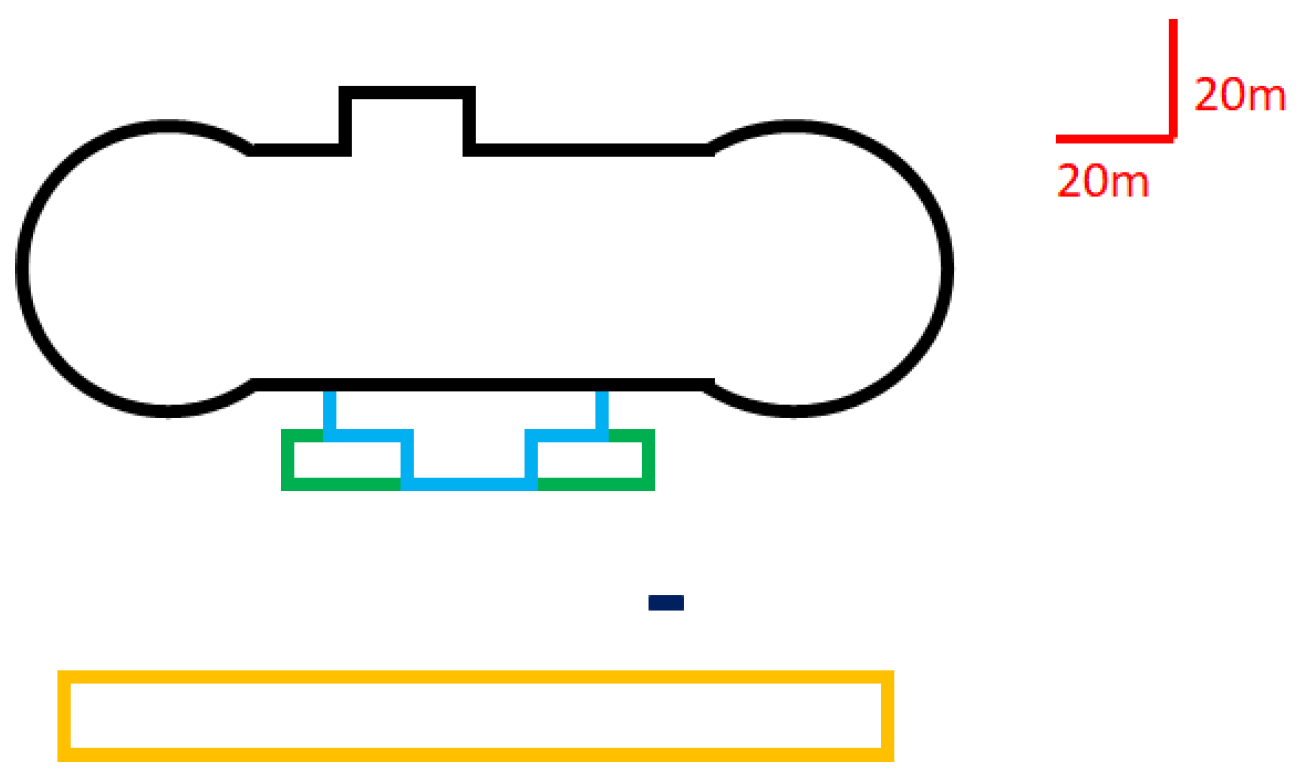
\includegraphics[width=0.7\linewidth]{Chapter5/Figs/Raster/wylfaTraceNew.png}
 \captionof{figure}{The position of the detector (dark blue) shown to scale compared with the main reactor building (black) with the secondary reactor buildings shown (cyan and green) which are of differing heights. The turbine hall (orange) is behind the detector.} %~can be used as a kind of place holder in latex
 \label{fig:wylfaTrace}
\end{figure}

\begin{figure}[H]
 \centering
 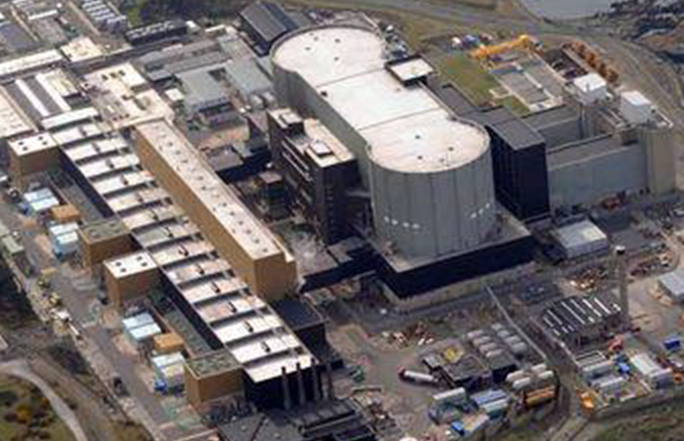
\includegraphics[width=0.7\linewidth]{Chapter5/Figs/Raster/wylfaArielView.png}
 \captionof{figure}{An aerial view of the Wylfa power station the main reactor building is the the shape of a "dog bone" the detector was placed in-between the turbine hall and reactor building.} %~can be used as a kind of place holder in latex
 \label{fig:wylfaAir}
\end{figure}

\section{Simulation Of Cosmic $\mu$s }\label{sec:SimulationOfCosmics}
Before the data could be analysed a simulation of cosmic $\mu$ using a cosmic hemisphere was used in order to quantify segmentation effects and any other detector effects. These can be quite significant as seen in figures \ref{fig:phiGenVsRecoHem} and \ref{fig:cirPhiGenVsRecoHem} the reconstruction of our detector can be quite adversely effected by vertical events. If an event is vertical in one side of the detector then the other side will dominate as such it results in spikes at 0$^\circ$, 90$^\circ$, 180$^\circ$, 270$^\circ$. This bin migration is expected due to its evenness it should not have a significant effect on the shadows. 
\\\\ However this is only true with $\phi$, in $\theta$ this is significantly less pronounced as seen in figure \ref{fig:thetaGenVsRecoHem} the reconstruction of $\theta$ is mostly quite accurate with only a few of the 
\begin{figure}[H]
 \centering
 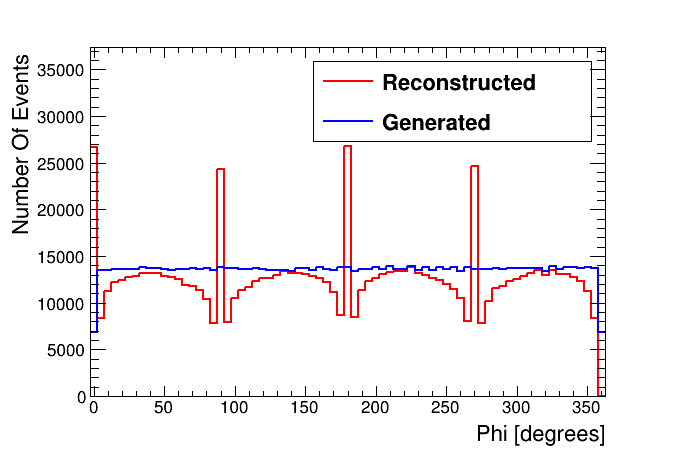
\includegraphics[width=0.8\linewidth]{Chapter5/Figs/Raster/hemispherePhiCompare.png}
 \captionof{figure}{Generated $\phi$ vs reconstructed $\phi$ with the online track fitter for a cosmic hemisphere distribution} %~can be used as a kind of place holder in latex
 \label{fig:phiGenVsRecoHem}
\end{figure}

\begin{figure}[H]
 \centering
 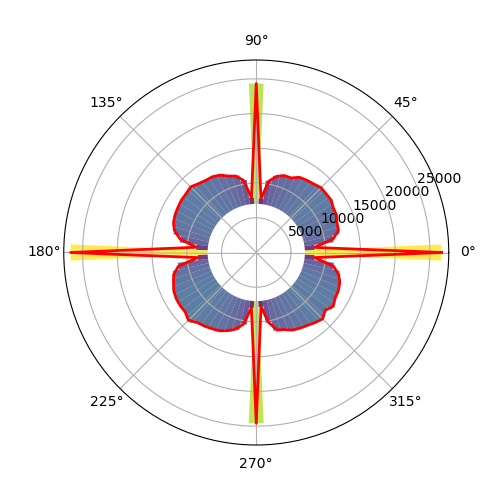
\includegraphics[width=0.6\linewidth]{Chapter5/Figs/Raster/cosmicSimpleHemNoDead_Ciruclarphi.png}
 \captionof{figure}{Circular plot of the reconstructed $\phi$ for a simulated cosmic hemisphere.} %~can be used as a kind of place holder in latex
 \label{fig:cirPhiGenVsRecoHem}
\end{figure}


\begin{figure}[H]
 \centering
 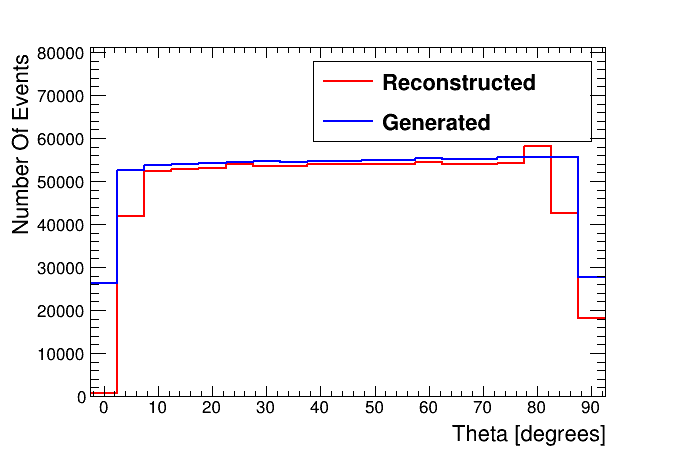
\includegraphics[width=0.8\linewidth]{Chapter5/Figs/Raster/hemisphereThetaCompare.png}
 \captionof{figure}{Generated $\theta$ vs reconstructed $\theta$ for a cosmic hemisphere distribution} %~can be used as a kind of place holder in latex
 \label{fig:thetaGenVsRecoHem}
\end{figure}

\begin{figure}[H]
 \centering
 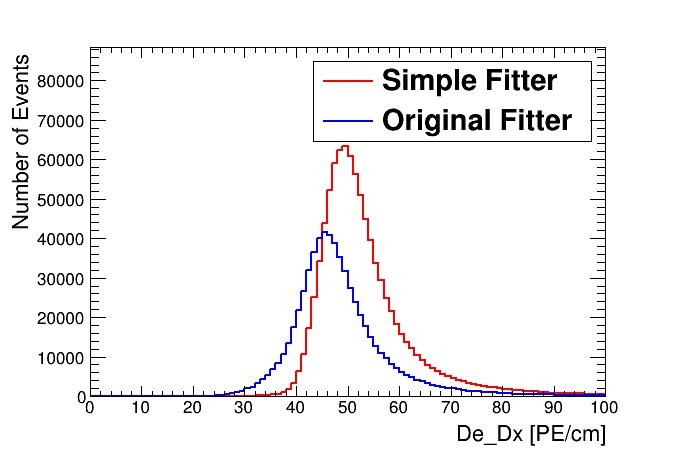
\includegraphics[width=0.8\linewidth]{Chapter5/Figs/Raster/dedxComarison.png}
 \captionof{figure}{\hl{need to add in generated de dx for this ploy} This is also more a show of the $\chi^2$/DOF effects the dE/dx and therefore how that may or may not be useful for online use.} %~can be used as a kind of place holder in latex
 \label{fig:dedxGenVsRecoHem}
\end{figure}

\begin{figure}[H]
 \centering
 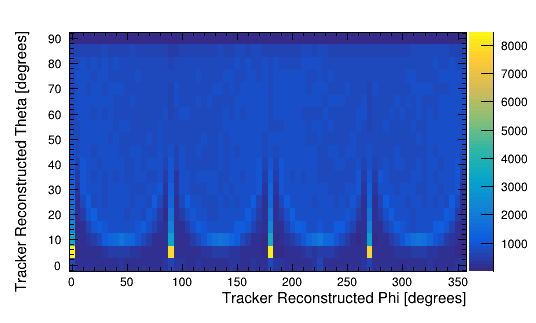
\includegraphics[width=0.8\linewidth]{Chapter5/Figs/Raster/phi_vs_theta_hem_simNoDead.png}
 \captionof{figure}{\hl{theta has been reversed now!!!} Simulated cosmic hemisphere which has a flat distribution in $\theta$ from 0$^\circ$ to 90$^\circ$ and a flat distribution in $\phi$ from 0$^\circ$ to 360$^\circ$ which is then reconstructed using the online track fitter} %~can be used as a kind of place holder in latex
 \label{fig:simulatedHemisphereDist}
\end{figure}

\begin{figure}[H]
 \centering
 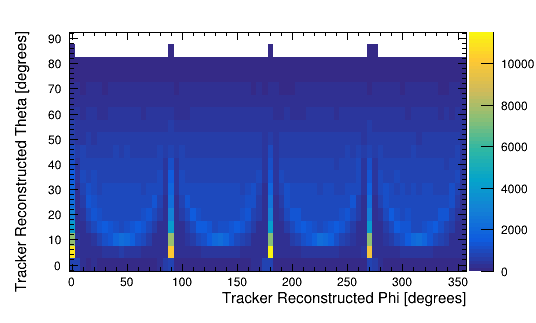
\includegraphics[width=0.8\linewidth]{Chapter5/Figs/Raster/simulatedNormalDistirbution.png}
 \captionof{figure}{\hl{theta has been reversed now!!!} Simulated distribution with an ideally generated cosmic distribution.} %~can be used as a kind of place holder in latex
 \label{fig:simulatedNormalDist}
\end{figure}

\section{Reactor Shadow: Methodology} \label{sec:ReactorShadowMethodology}

\begin{figure}[H]
 \centering
 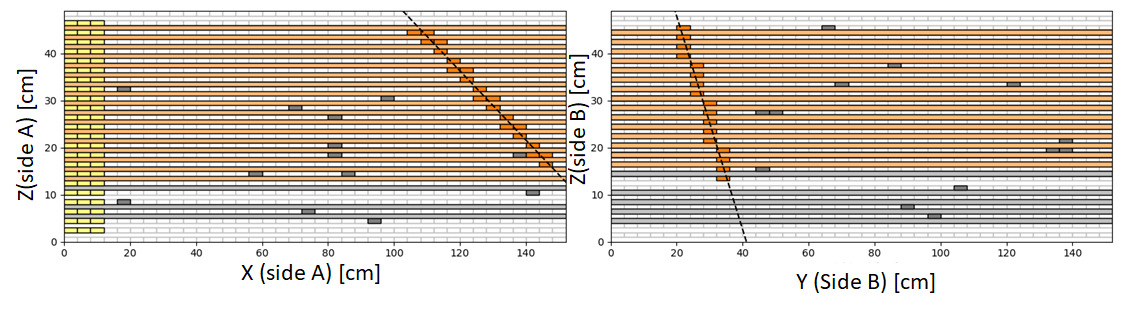
\includegraphics[width=\linewidth]{Chapter5/Figs/Raster/3000ExampleEvent.png}
 \captionof{figure}{An example event from the Wylfa deployment the cosmic enters through the top of the detector and exits through side A. Bars that are in signal are shown in orange bars that are noise are shown in grey, with un-instrumented channels shown in yellow on side A.} 
 \label{fig:3000ExampleEvent}
\end{figure}

\begin{figure}[H]
 \centering
 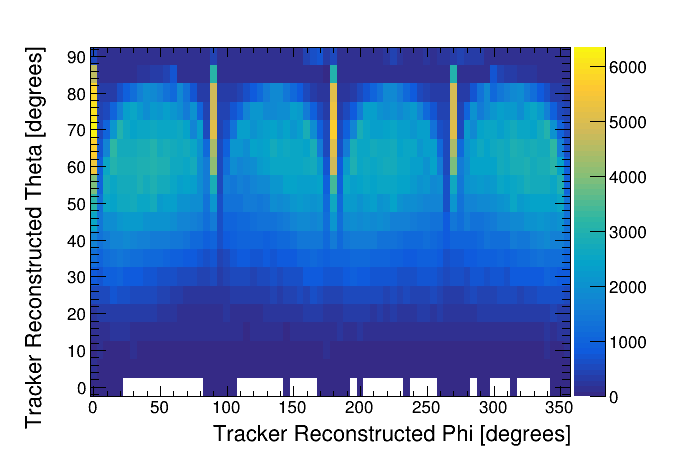
\includegraphics[width=0.8\linewidth]{Chapter5/Figs/Raster/pVsTWylfaReversed.png}
 \captionof{figure}{Measured $\theta$ and $\phi$ from the cosmic muons from the Wylfa deployment, the reactor is at $\sim$ 90$^{\circ}$. The turbine hall is at $\sim$ 270$^{\circ}$.} 
 \label{fig:pVsTWylfaReversed}
\end{figure}

\begin{figure}[H]
 \centering
 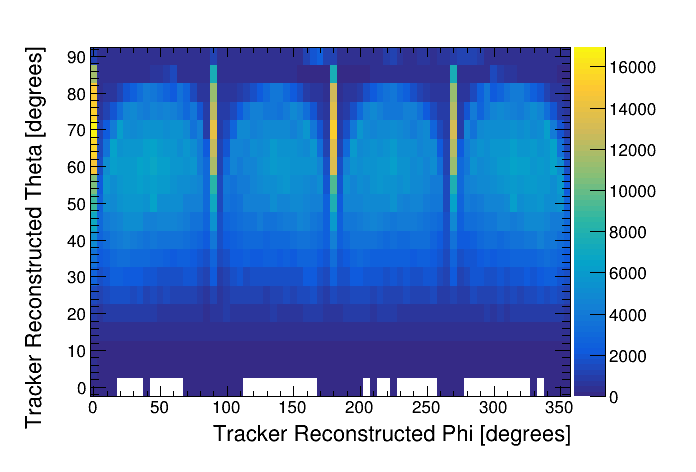
\includegraphics[width=0.8\linewidth]{Chapter5/Figs/Raster/pVsTLiverpoolReversed.png}
 \captionof{figure}{Measured $\theta$ and $\phi$ from the cosmic muons from the Liverpool deployment.} 
 \label{fig:pVsTLiverpoolReversed}
\end{figure}

\begin{figure}[H]
\centering
\begin{subfigure}{.5\textwidth}
  \centering
  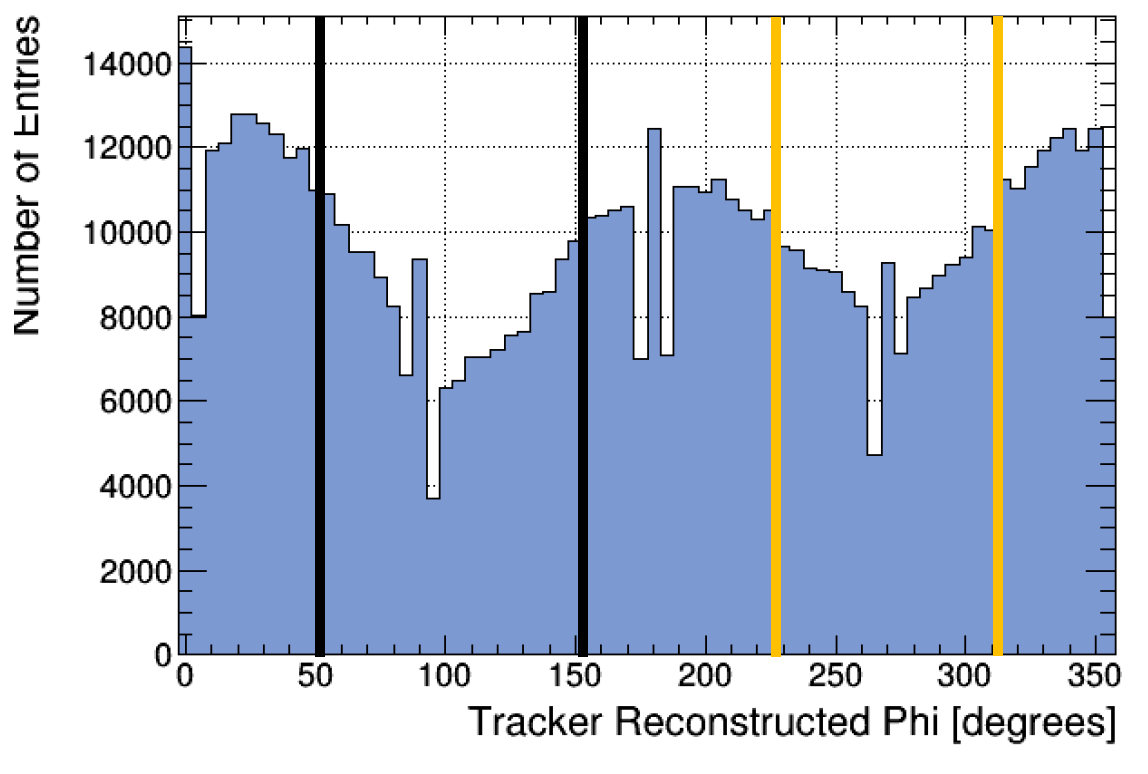
\includegraphics[width=\linewidth]{Chapter5/Figs/Raster/linReversedWylfaSlice0-57.5.png}
  \captionsetup{width=.9\linewidth}
  \caption{Linear histogram showing the dips in the shadows from the shadows of the reactor buildings and turbine halls.}
  \label{subFig:linReversedWylfaSlice0-57.5}
\end{subfigure}%
\begin{subfigure}{.5\textwidth}
  \centering
  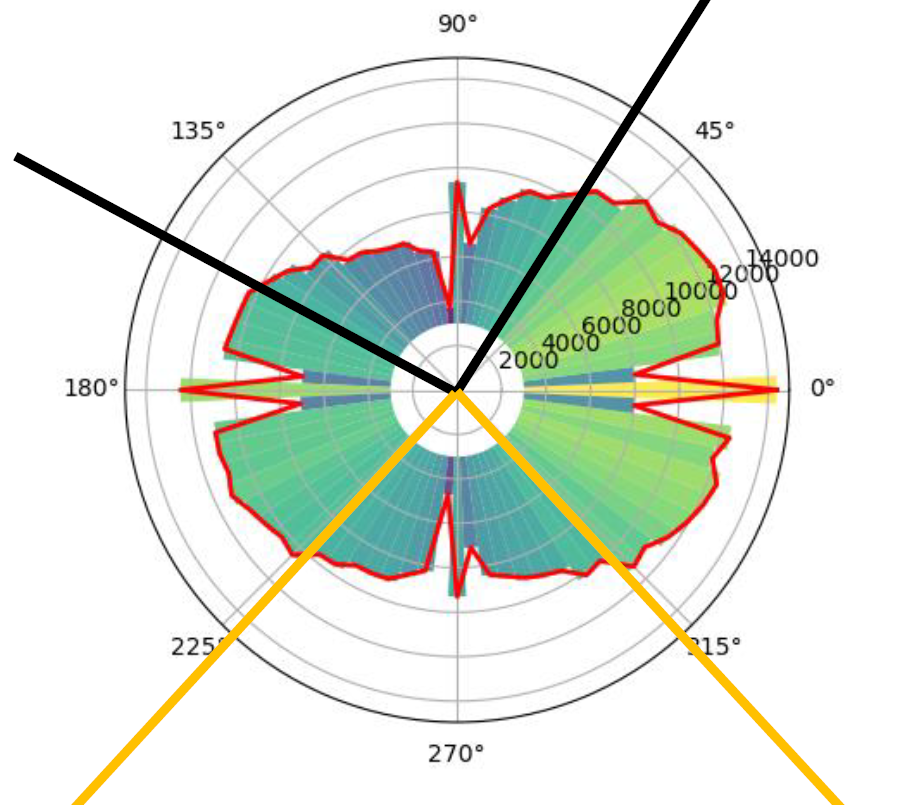
\includegraphics[width=0.765\linewidth]{Chapter5/Figs/Raster/cirReversedWylfaSlice0-57.5.png}
  \captionsetup{width=.9\linewidth}
  \caption{Circular histogram showing the dips in the shadows from the shadows of the reactor buildings and turbine halls.}
  \label{subFig:linReversedWylfaSlice0-57.5}
\end{subfigure}
\caption{Histograms showing how the shadows of the reactor buildings and the turbine hall are cast on to the detector from $\theta$ of 0$^\circ$ to 57.5$^\circ$. The Reactor buildings are shown in-between the black lines the turbine hall is shown in-between the orange lines.}
\label{fig:WylfaSlice0-57.5}
\end{figure}

\begin{figure}[H]
 \centering
 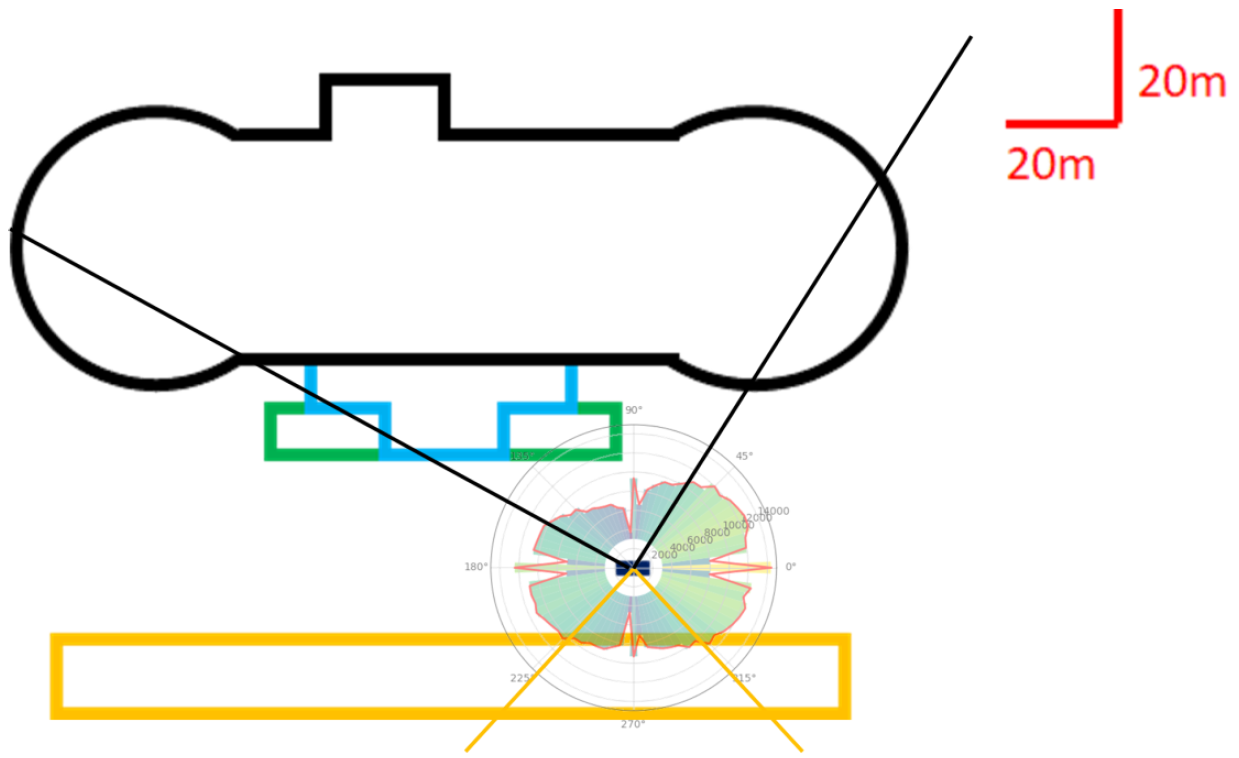
\includegraphics[width=\linewidth]{Chapter5/Figs/Raster/cirOverlayReversedWylfaSlice0-57.5.png}
 \captionof{figure}{The circular distribution of the $\phi$ from a $\theta$ of 0$^\circ$ - 57.5$^\circ$ the tower closest to the detector is dominating the distribution of the shadow.} %~can be used as a kind of place holder in latex
 \label{fig:wylfaTraceAbove32.5}
\end{figure}

\begin{figure}[H]
\centering
\begin{subfigure}{.5\textwidth}
  \centering
  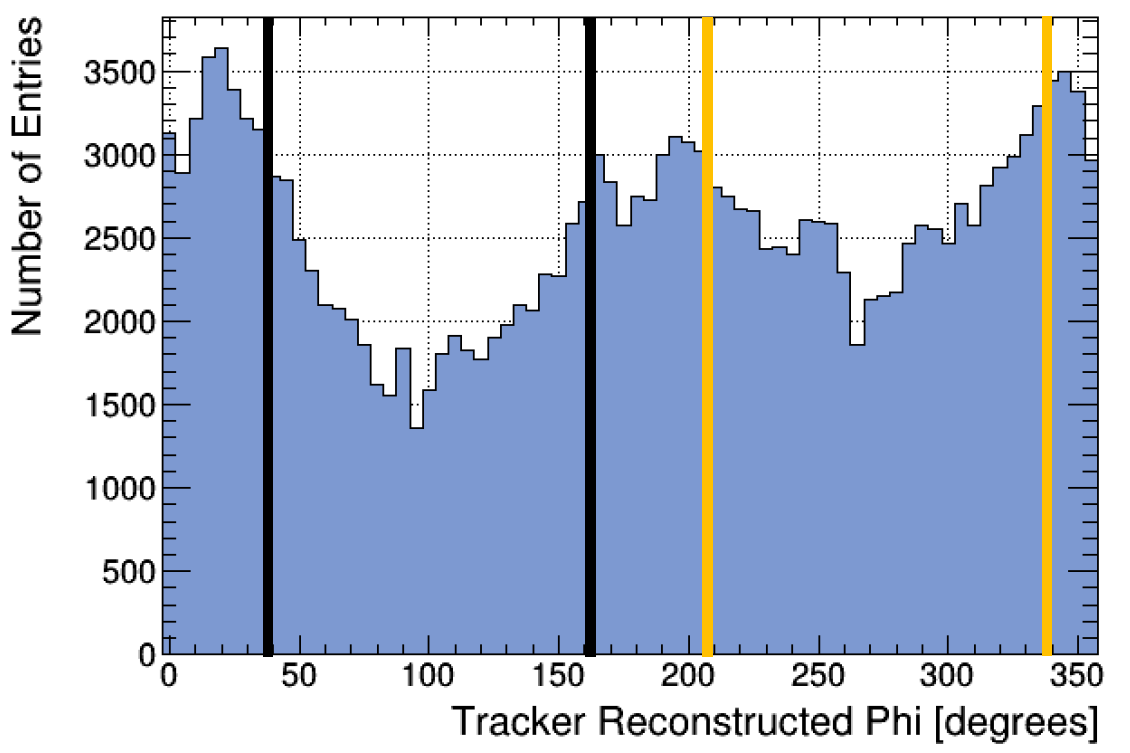
\includegraphics[width=\linewidth]{Chapter5/Figs/Raster/linReversedWylfaSlice0-37.5.png}
  \captionsetup{width=.9\linewidth}
  \caption{Linear histogram showing the dips in the shadows from the shadows of the reactor buildings and turbine halls.}
  \label{subFig:linReversedWylfaSlice0-37.5}
\end{subfigure}%
\begin{subfigure}{.5\textwidth}
  \centering
  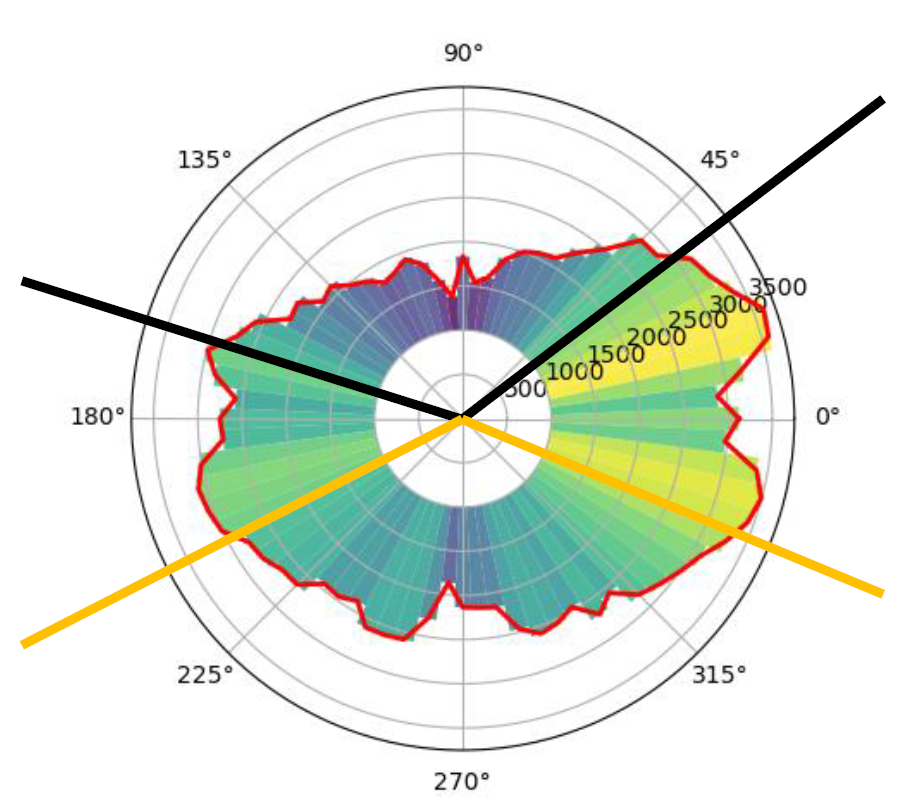
\includegraphics[width=0.765\linewidth]{Chapter5/Figs/Raster/cirReversedWylfaSlice0-37.5.png}
  \captionsetup{width=.9\linewidth}
  \caption{Circular histogram showing the dips in the shadows from the shadows of the reactor buildings and turbine halls.}
  \label{subFig:cirReversedWylfaSlice0-37.5}
\end{subfigure}
 \caption{Histograms showing how the shadows of the reactor buildings and the turbine hall are cast on to the detector from $\theta$ of 0$^\circ$ to 37.5$^\circ$. The Reactor buildings are shown in-between the black lines the turbine hall is shown in-between the orange lines.}
\label{fig:WylfaSlice0-37.5}
\end{figure}

\begin{figure}[H]
 \centering
 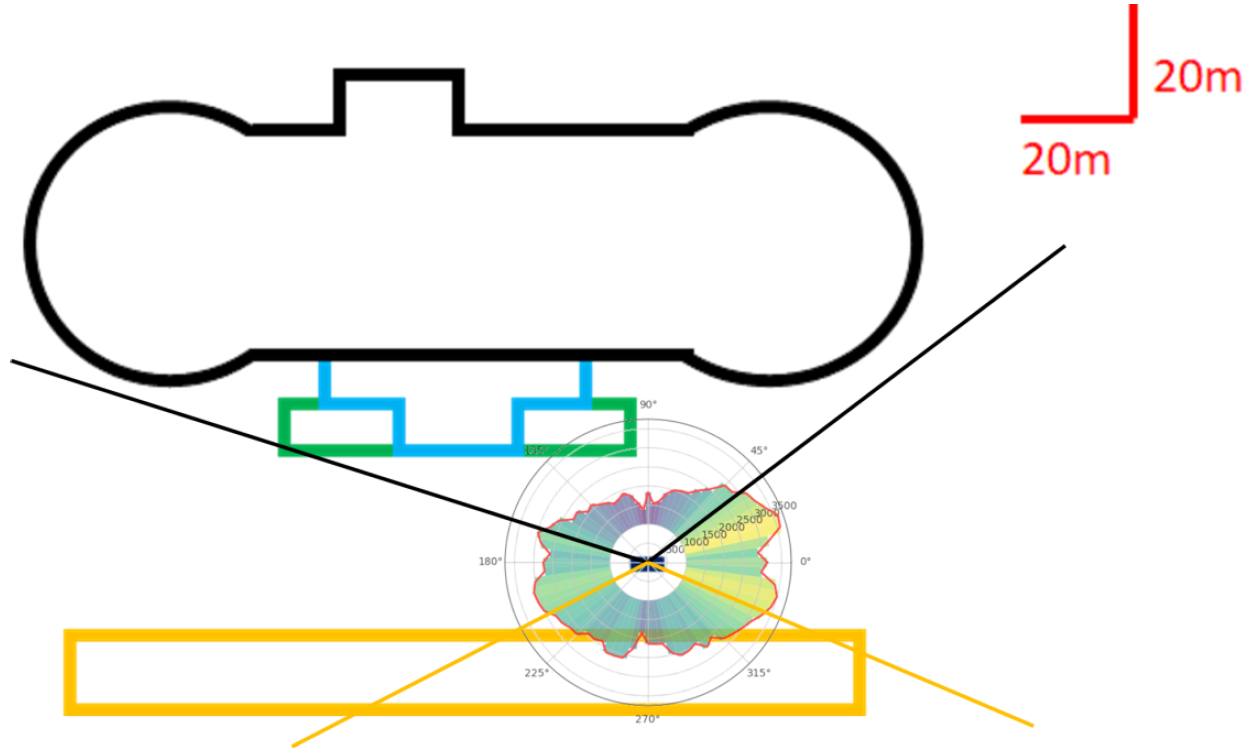
\includegraphics[width=\linewidth]{Chapter5/Figs/Raster/cirOverlayReversedWylfaSlice0-37.5.png}
 \captionof{figure}{The circular distribution of the $\phi$ from a $\theta$ of 0$^\circ$ 37.5$^\circ$ the reactor shadow is now dominated by the main reactor building.} %~can be used as a kind of place holder in latex
 \label{fig:wylfaTraceAbove52.5}
\end{figure}

\begin{figure}[H]
 \centering
 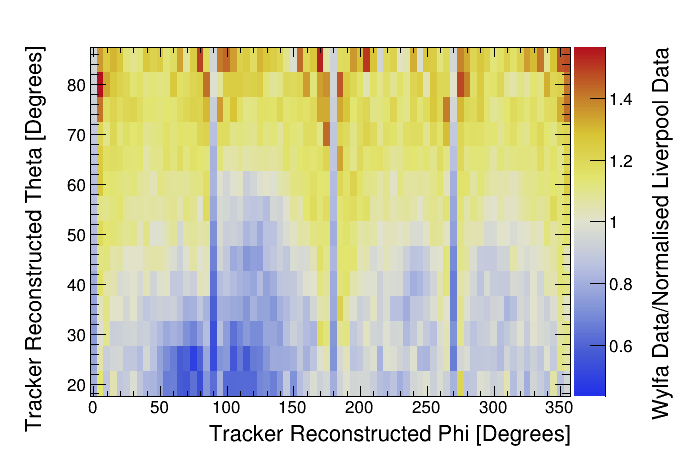
\includegraphics[width=1.0\linewidth]{Chapter5/Figs/Raster/wylfaToLiverpoolRatioDynamic17.5-87.5.png}
 \captionof{figure}{The ratio of the Wylfa $\theta$ and $\phi$ cosmic muon distribution divided by the Liverpool $\theta$ and $\phi$ cosmic muon distribution. The Liverpool data is normalised to the Wylfa data. The ratio minimum $\sim$ 0.5 represents a deficit (attenuation) of $\sim$ 50\,$\%$. The maximum ratio $\sim$ 1.5 represents an excess of $\sim$ 50\,$\%$.} %~can be used as a kind of place holder in latex
 \label{fig:wylfaDivLiverpool}
\end{figure}

\begin{figure}[H]
\centering
\begin{subfigure}{.5\textwidth}
  \centering
  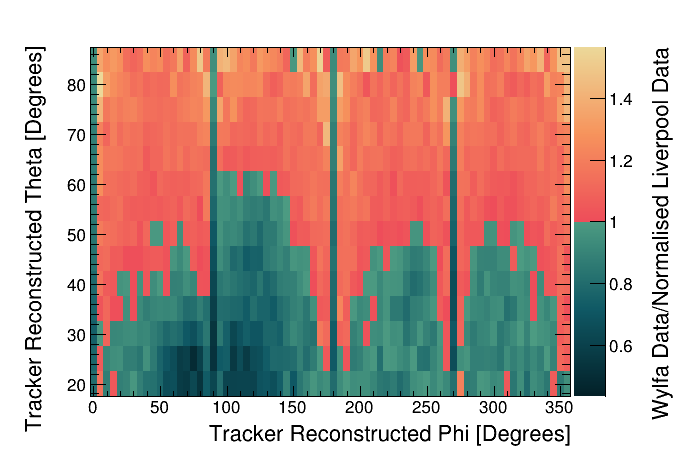
\includegraphics[width=\linewidth]{Chapter5/Figs/Raster/WylfaToLiverpoolRatio_starkMap.png}
  \captionsetup{width=.9\linewidth}
  \caption{``Stark'' colour map .}
  \label{subFig:wylfaToLiverpoolRatioStarkMap}
\end{subfigure}%
\begin{subfigure}{.5\textwidth}
  \centering
  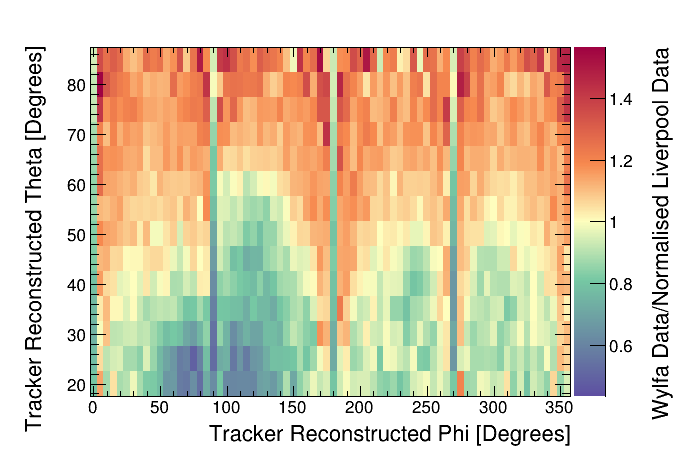
\includegraphics[width=\linewidth]{Chapter5/Figs/Raster/WylfaToLiverpoolRatio_sanRbMap.png}
  \captionsetup{width=.9\linewidth}
  \caption{``Sanitised'' rainbow colour map.}
  \label{subFig:wylfaToLiverpoolRatioSanRbMap}
\end{subfigure}
\caption{Alternative colour maps for figure \ref{fig:wylfaDivLiverpool}. }
\label{fig:wylfaToLiverpoolRatioCustomMaps}
\end{figure}

\begin{figure}[H]
 \centering
 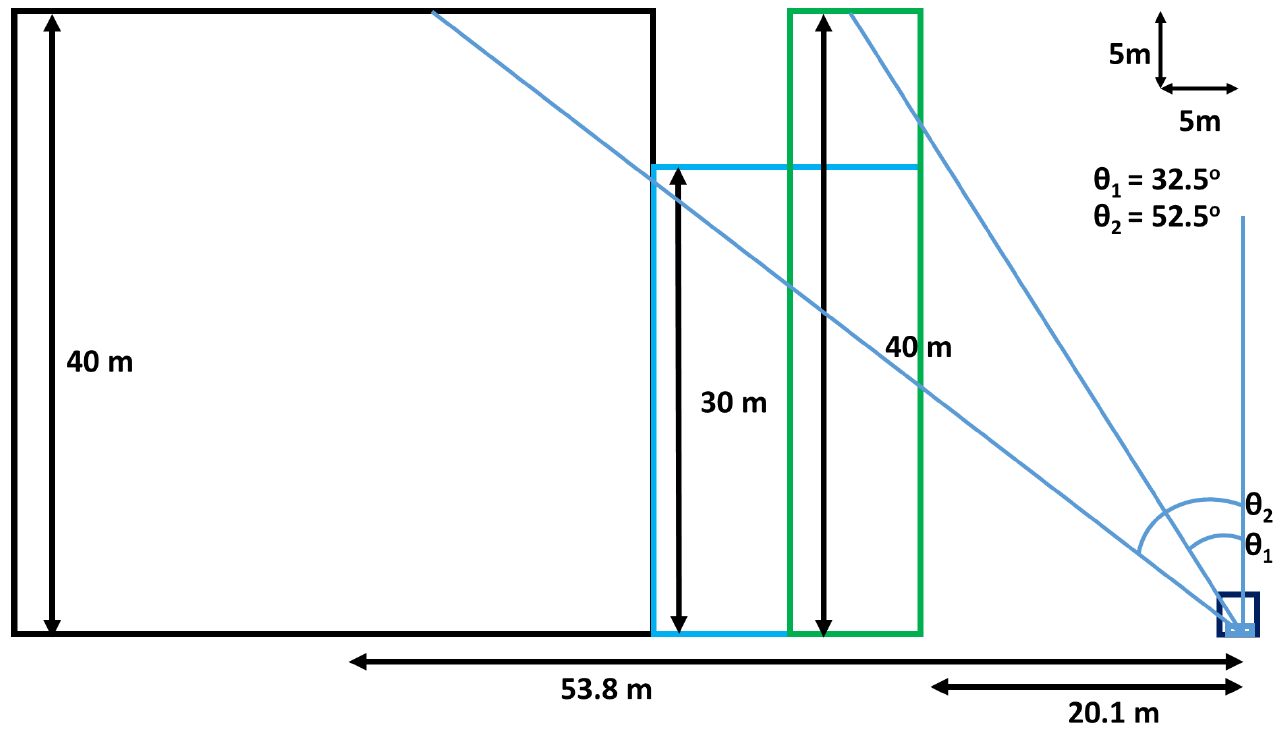
\includegraphics[width=1.0\linewidth]{Chapter5/Figs/Raster/wyflaHieghtsNew.png}
 \captionof{figure}{The estimated heights of the reactor buildings, above 32.5$^{\circ}$ the green tower closest to the detector dominates, above 52.5$^{\circ}$ the main reactor building dominates the shadow.} %~can be used as a kind of place holder in latex
 \label{fig:wylfaHieghts}
\end{figure}

\begin{figure}[H]
\centering
\begin{subfigure}{.5\textwidth}
  \centering
  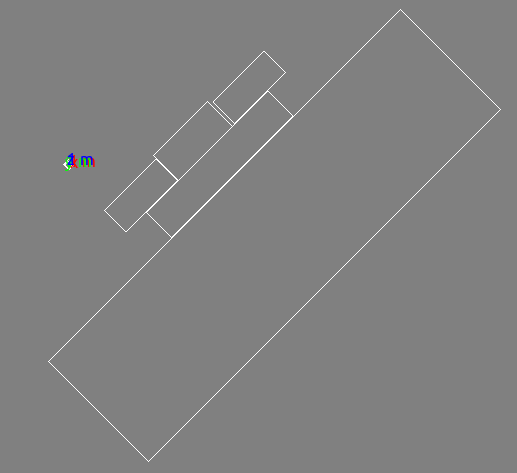
\includegraphics[width=0.685\linewidth]{Chapter5/Figs/Raster/reactorBuildingsTopDown.png}
  \captionsetup{width=.9\linewidth}
  \caption{Top down perspective of simulated reactor buildings in Geant4.}
  \label{subFig:simulatedReactorBuildingsTopDown}
\end{subfigure}%
\begin{subfigure}{.5\textwidth}
  \centering
  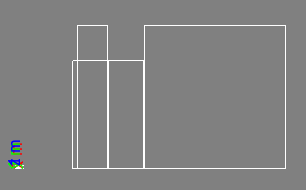
\includegraphics[width=\linewidth]{Chapter5/Figs/Raster/reactorBulidingsDepth.png}
  \captionsetup{width=.9\linewidth}
  \caption{Side on Perspective of simulated reactor buildings in Geant4.}
  \label{subFig:simulatedReactorBuildingsDepth}
\end{subfigure}
\caption{The reactor buildings simulated in Geant 4 next to the detector which is at the origin.}
\label{fig:simulatedReactorBuildings}
\end{figure}


\begin{figure}[H]
 \centering
 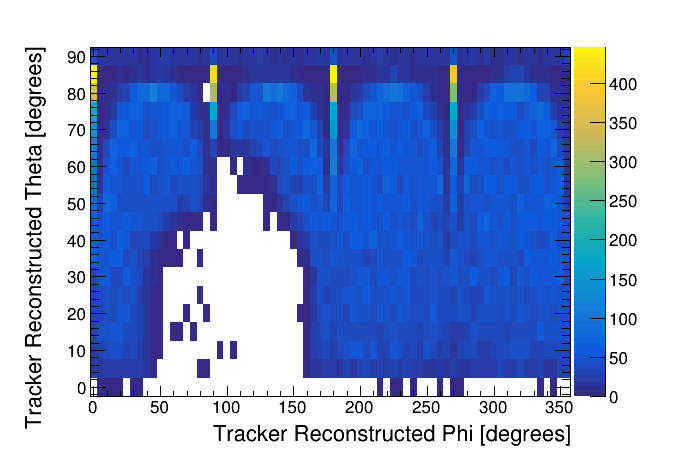
\includegraphics[width=0.8\linewidth]{Chapter5/Figs/Raster/pVsTReactorAllReversed.png}
 \captionof{figure}{The simulated reactor shadow assuming the heights calculated from figures \ref{fig:wylfaDivLiverpool} and \ref{fig:wylfaHieghts} and assuming that each building is made from 100\,\% concrete.} 
 \label{fig:simulatedShadowDist}
\end{figure}

% end